\section{The Logistic Map as a Model for Population Growth}

One-dimensional recursive equations $x_{n+1} = f(x_n)$ are used for modelling various dynamical systems. 
Notwithstanding their simplicity, many of these maps exhibit extremely complicated properties which are also present in their more complicated counterparts.

Consider, for example, bacteria population in discrete time intervals. 
If the population is low and resource abundant, the rate of growth is in proportion to the population, which gives rise to the following equation
\begin{equation}\label{eq:1d iterative map}
p_{t+1} = p_{t} b,
\end{equation}
where $p_{t}$ is the population of the bacteria at the discrete time $t$ and $b$, as a constant, is the static birth rate for bacteria whose value will depend on the model.

The limited resource will slow down the rate of growth of the bacteria as the population increases, and the relation will become 
\begin{equation}\label{eq:p times beff}
	p_{t+1} =  p_{t} \be
\end{equation}

The usual assumption is that $\be$ is close to $b$ when the population is low, and there is a threshold above which the population will decrease. 
At the threshold $\be$ will be zero.

The simplest equation for modelling $\be$ is the linear equation
\begin{equation} \label{eq:b_effective}
\be = b - ap,
\end{equation}
where $a$ is another constant depending on the model.
Combining the equations \eqref{eq:p times beff} and \eqref{eq:b_effective}, the recursive formula becomes 
$$
p_{t+1}  = b p_t - ap_t^2
$$

Substituting $p_{t} := \frac{b}{a} x_{t}, \lambda := \frac{b}{4}$, we obtain
$$
x_{t+1} = 4 \lambda x_t(1-x_t) 
$$
Thence comes the standard forms of the logistic map depending on one variable $\lambda$
\footnote{
Some sources defined the logistic map as $L^*_{\lambda}(x) = \lambda x(1-x)$ without the constant 4. 
In this report, however, we will use equation \ref{eq_logistic}, which has the advantage that the maximum value attained by $\L(x)$ at $\frac{1}{2}$ is $\lambda$, and it will also be consistent to the definitions of other class of functions discussed later in the report.
}
\begin{equation}\label{eq_logistic}
	L_{\lambda}(x) = 4 \lambda x(1-x)
\end{equation}

% graph produced by `logistic_map_diff_lambda`
\begin{figure}[t]
	\centering
	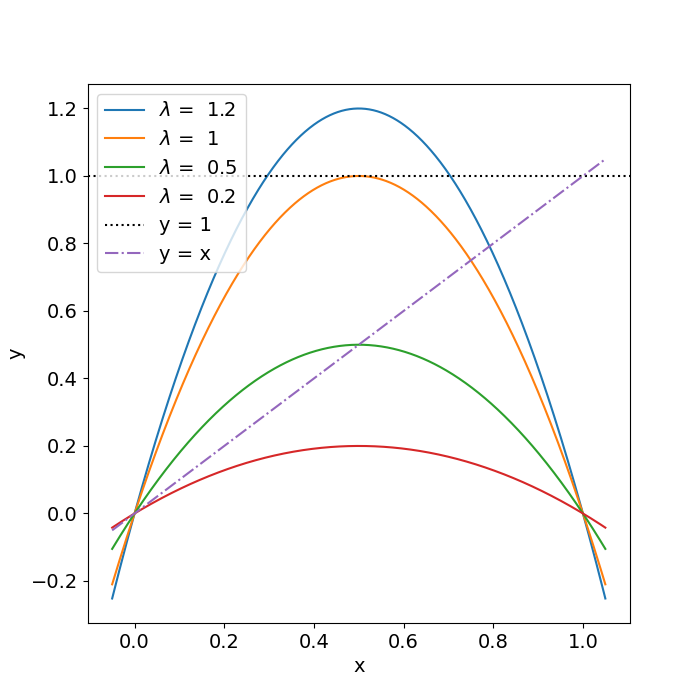
\includegraphics[width=0.7\textwidth]{./figures/logistic_map_diff_lambda.png}
	\caption{Graphs of logistic map $L_{\lambda}(x) = 4 \lambda x(1-x)$ for different $\lambda$ compared with the line $y=x$ and $y = 1$.} 
	\label{fig:logistic_map_diff_lambda}
\end{figure}

% The dynamical system in discrete time interval generated by the iterations of the logistic map is the study of this session.

Scrutinising the class of discrete logistic functions plotted in figure \ref{fig:logistic_map_diff_lambda}, some of their properties are obvious:

\begin{enumerate}
	\item $\L(x)$ is a smooth function;
	\item $\L(x)$ concaves downwards, that is, $\L(x)'' < 0$;
	\item $\L(x)$ attains a unique maximum at $x = \frac{1}{2}$, and $L_{\lambda}(\frac{1}{2}) = \lambda$; and,
	\item when $0 \leq \lambda$ and $x$ is restricted to the domain $[0, 1]$, $\L(x)$ is a two-to-one non-surjective (except for $\lambda = 1$) function $\L(x): [0,1] \rightarrow [0,\lambda]$. 
\end{enumerate}


We can check if this model would work as expected by comparing it to its continuous counterpart 
\begin{equation}\label{eq_logistic_continuous}
	\frac{dp}{dx} = c p(x) (1-p(x)),
\end{equation}

where $c$ is some arbitrary constant denoting the rate of growth. 
The unique solution to this ordinary differential equation with the initial condition $p(0) = \frac{1}{2}$ is 
$$
p(x) = \frac{e^{cx}}{1+e^{cx}}.
$$
\begin{figure}
	\centering
	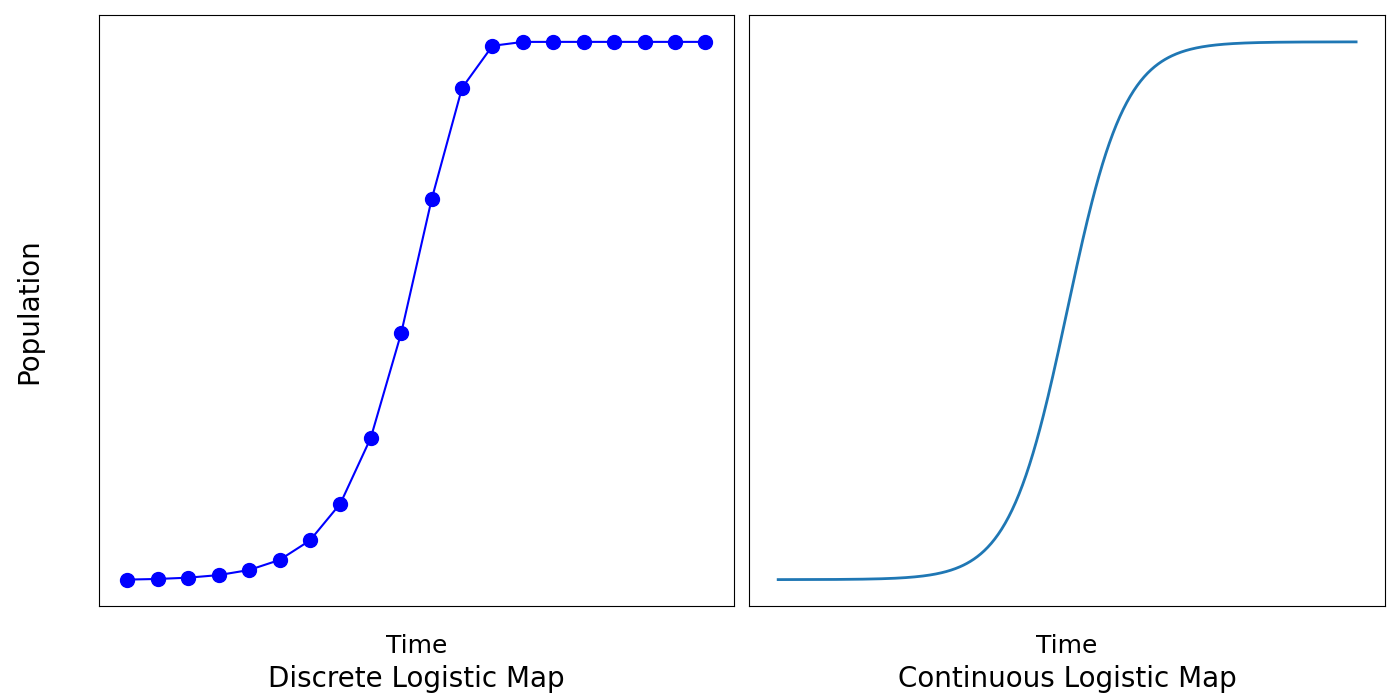
\includegraphics[width=0.8\textwidth]{./figures/con_vs_discrete_logistic_map.png}
	\caption{The population of the bacteria modelled by the discrete (left) v.s. continuous (right) logistic map. 
	The discrete case is modelled by $\lambda = 0.5$ and $x_0 = 0.0003$, and the continuous case has $c=1$.}
	\label{fig:con_vs_discrete}
\end{figure}
The graph of the populations modelled by \eqref{eq_logistic} and \eqref{eq_logistic_continuous} are shown in Figure \ref{fig:con_vs_discrete}.
Indeed, at least for the selected value of $\lambda$ and $c$, the population modelled by the two maps are similar.

Having settled that the discrete logistic map is a good simplification for the already-simplified equation \eqref{eq_logistic_continuous} as a model for population growth, you may wonder why we bother studying such a simple equation. 
The reason is, as simple as it seems, that the iteration of equation \eqref{eq_logistic} gives rise to some extremely complicated dynamical systems with many surprising properties. 
These interesting dynamics are also observed in the continuous case and is the study of the next session.

It shall be stressed, at the end of this session before we go in depth into the theoretical discussions, that no impression shall be made to assume that one-dimensional discrete iterative maps are only useful as a crude model for bacteria population growth. 
There are abundant examples where equation \eqref{eq:1d iterative map} can be used as a model, some up to a strikingly high accuracy. 
For example: in genetics, it is used when investigating on the frequency of the genotype \cite{genotype}; in economics, modelling the relationship between commodity quantity and price \cite{economics}; and in social science, on the propagation of rumours \cite{social_science}, among many others.


\section{Logistic Bifurcations}

To make our terminology precise and avoid any possible confusion, we shall reiterate that the focus of this session is the one-dimensional discrete dynamical system depending on one parameter $\lambda$, generated by the iterations of the logistic map. 
Explicitly, it is the sequence $x_0, x_1, \dots$, where $x_0$ is the initial condition, and $x_{n+1} = \L(x_n)$, as defined in \eqref{eq_logistic}.

The first step of studying this system is to plot it with different initial values $x$ and parameters $\lambda$. Only $0 \leq \lambda \leq 1$ and $0 \leq x_0 \leq 1$ are considered, so that $\L(x)$ is a map from $[0,1]$ to $[0,1]$. 

% graph produced by `modelling_pop_with_diff_logistic_maps` in `graph_qc` repo
\begin{figure}[htbp]
	\centering
	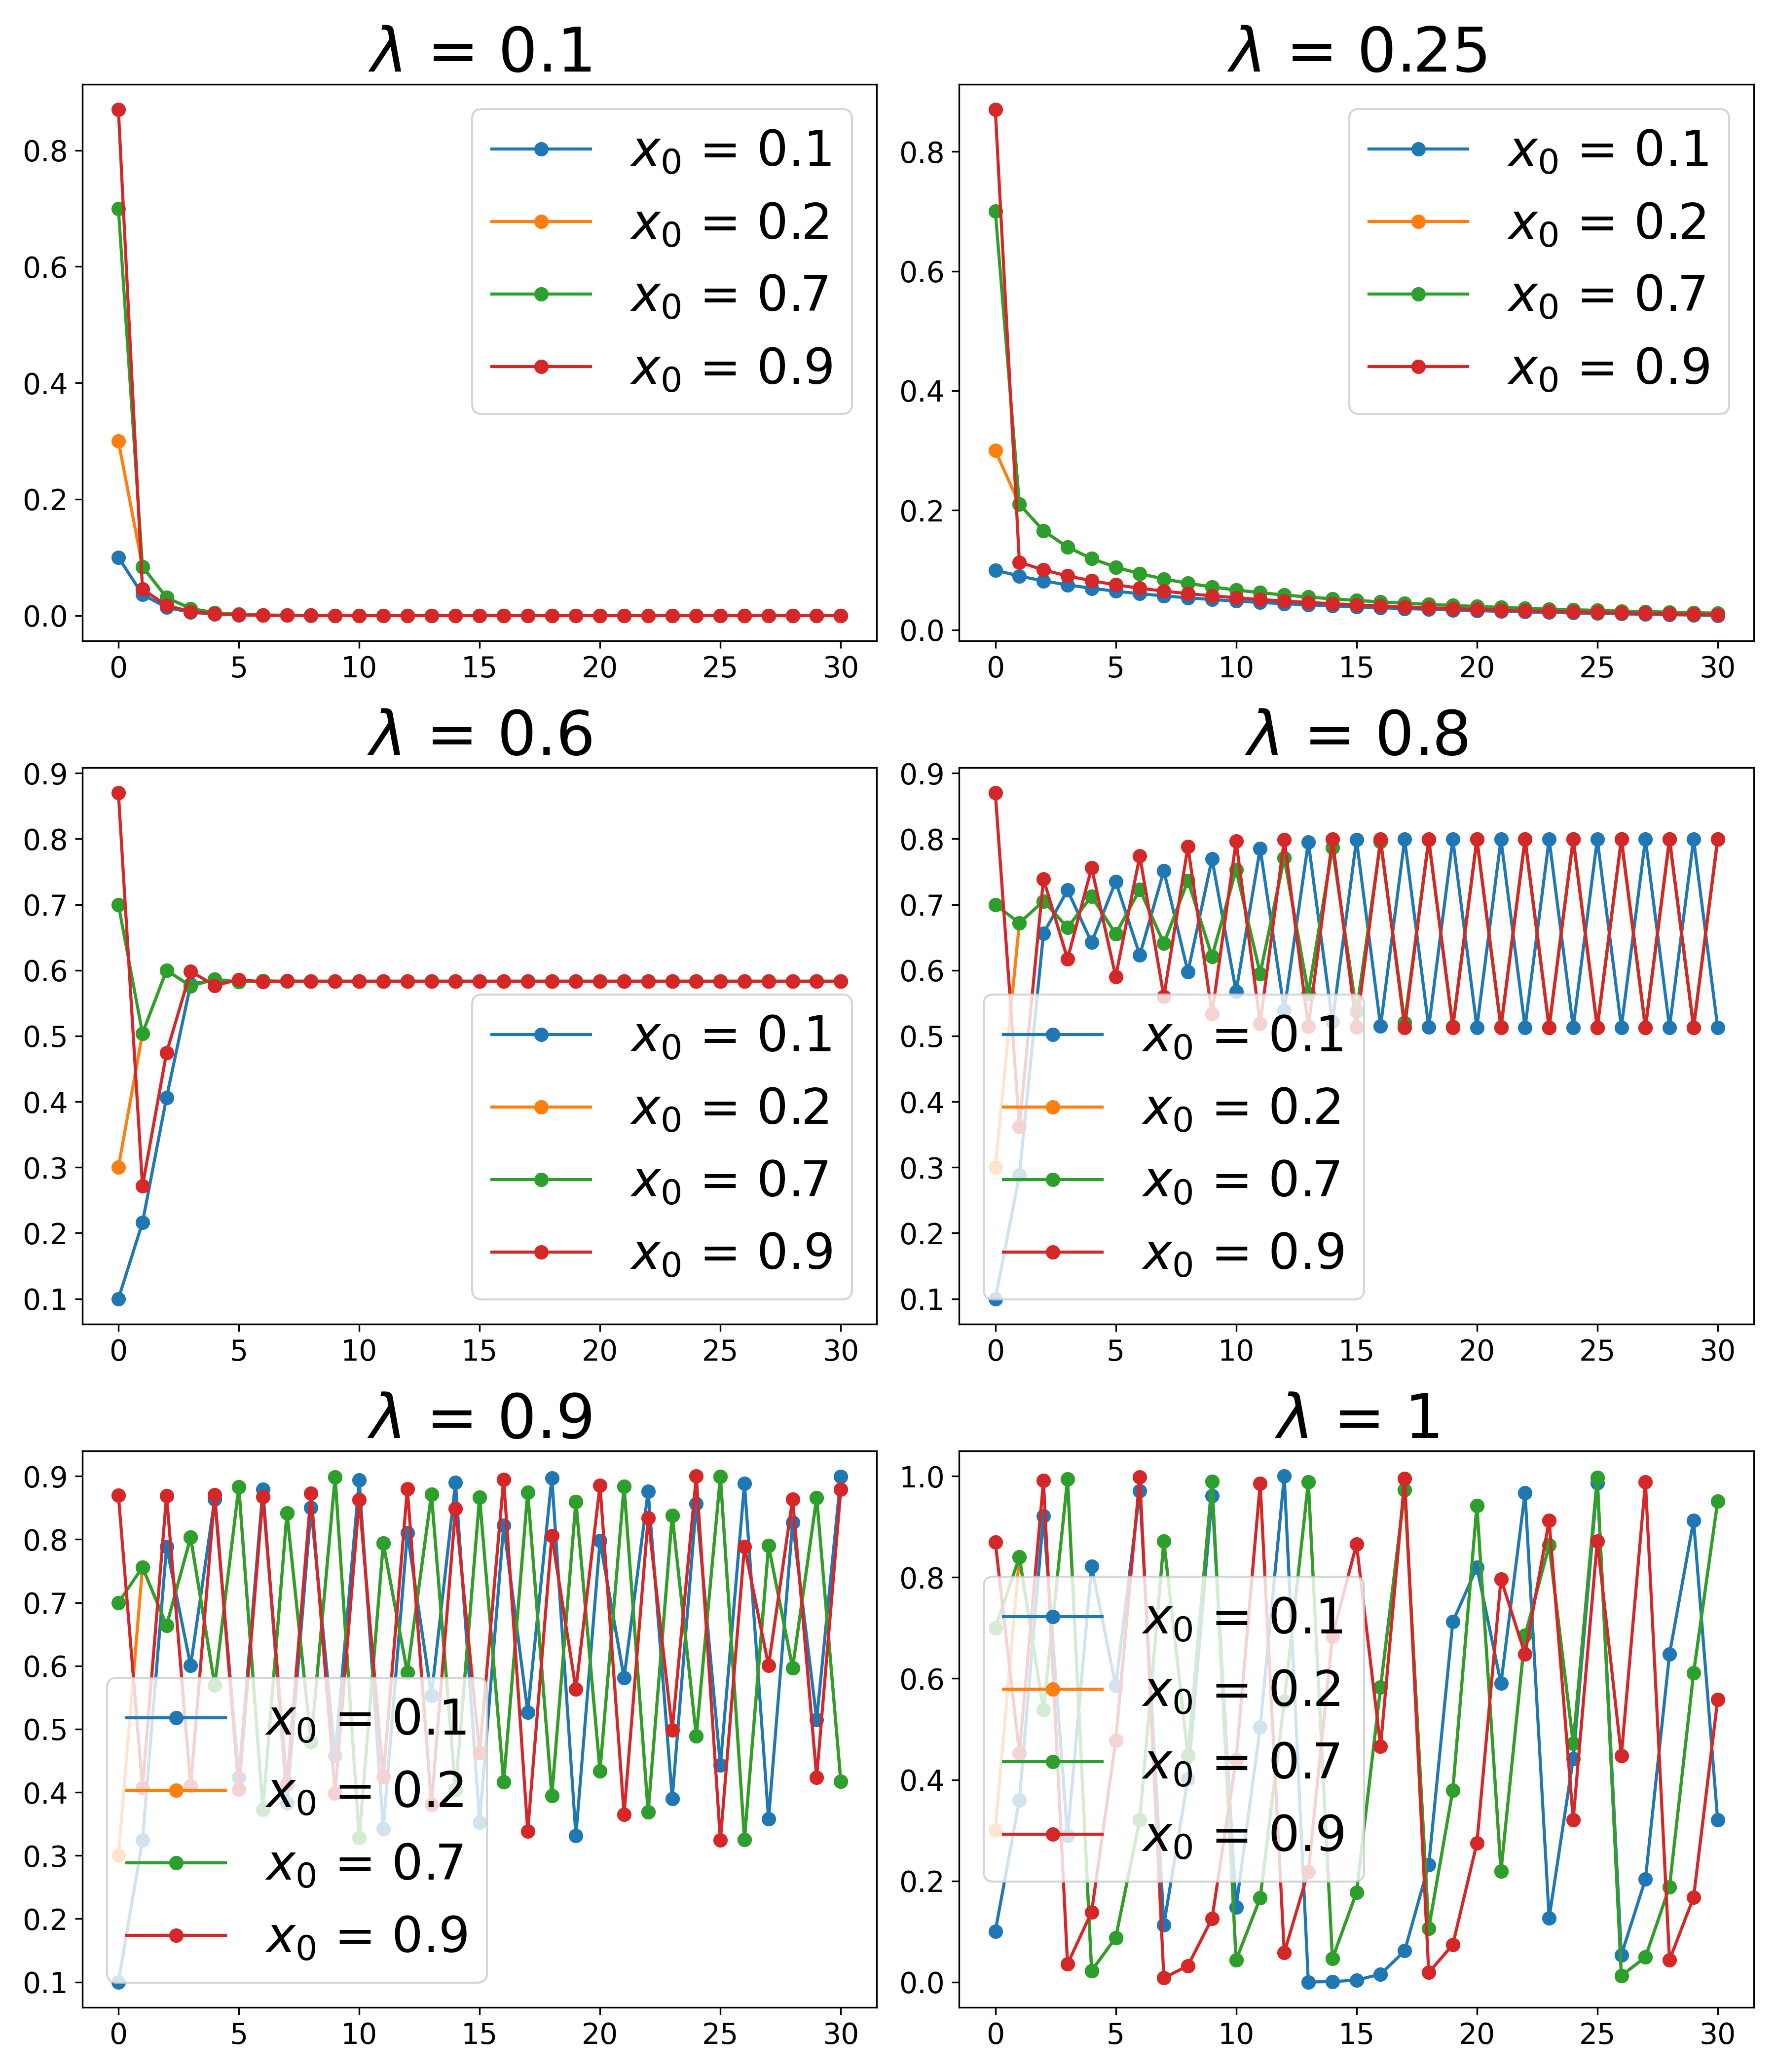
\includegraphics[width=0.9\textwidth]{./figures/various_iterating_logistic_map.png}
	\caption{Iterating the logistic map with different initial values and $\lambda$. All graphs are produced by setting a $x_0$ and $\lambda$, and iterating $x_{n+1} = L_{\lambda}(x_n)$, and plotting all $x_n$ values respect to iteration number $n$.}
	\label{fig:various_iter_logistic}
\end{figure}

There are several immediate observations upon looking at Figure \ref{fig:various_iter_logistic}.
When $\lambda = 0.1$ and $0.25$, it seems $\lim_{n \rightarrow \infty} x_n = 0$, regardless of the value of $x_0$.
For $\lambda = 0.6$, $\lim_{n \rightarrow \infty} x_n = l \neq 0$. 
(We can show that $l = \frac{7}{12}$ by Theorem \ref{th:_stable_unstable_fixed_point}.)

When $\lambda = 0.8$, $x_n$ no longer converges but oscillates in a stable two orbit. 
For $\lambda = 0.9$ and $\lambda = 1$, it is not clear if $x_n$ has any stable orbits or sensible patterns, and the best epithet for them would be `chaotic'.

For all cases, it seems like any initial condition, $x_0$, upon iteration, will eventually tend to some common dynamical behaviour depending only on $\lambda$.
The scatter plot in Figure \ref{fig:logistic bifurcation overview} is produced to capture the behaviour of $x_n$ as $n \rightarrow \infty$ for various intervals of $\lambda$.
These graphs are produced by picking a $\lambda$ and a random $x_0 \in [0,1]$, producing $x_{1} = \L(x_0), x_{2} = \L(x_1), \dots$ through thousands of iterations, ignoring the first several hundred $x_i$s, and plotting the rest of the $x_i$ on the coordinate $(x_i, \lambda)$. 
By repeating this process for one thousand equally spaced $\lambda \in [0,1]$, the bifurcation diagram is obtained.

These pictures of bifurcation are indeed spectacular. 
For $\lambda$ between $0$ and $a_0 = 0.25$, there is a stable fixed point $x = 0$.
When $\lambda$ becomes greater than $a_1 = 0.25$, $0$ is no longer the stable fixed point, but there is another unique stable fixed point greater than $0$.
Precisely when this stable fixed point becomes unstable, around $\lambda = a_2 \approx 0.77$, a stable two-cycle appears.
The stable two-cycle, again, disappears around $\lambda = a_3 \approx 0.86$, at which point a stable 4-cycle appears. 
This process of periodic doubling of the stable orbit, which seems to continue indefinitely, is denominated as \emph{periodic doubling bifurcation}.\footnote{
	The word bifurcation comes from medieval Latin bifurcātus, literally meaning two-forked. Here, it is used figuratively to describe the process of a single stable orbit forking into two.
	
	Bifurcations, in general, mean the change of the behaviour of dynamical systems as parameters vary.
	For systems depending only on one parameter, there are only three kinds of generic bifurcation: periodic doubling, tangent, and inverse periodic doubling \cite{Chaos_in_DS}.
	In this report, we will only touch on periodic doubling bifurcation.
	Bifurcation, in general, has very rich theory and is applicable to a large class of dynamical systems, including continuous ones and those of higher dimensions. \cite{dynamical_systems_v}.
}

Upon closer inspection of the sub-figures of Figure \ref{fig:logistic bifurcation overview}, zoomed around the windows of bifurcation, each stable orbit and bifurcation pattern seems to be self-similar, and all stable orbits cross the line $y = 0.5$ for some $\lambda$.

Periodic doubling bifurcations, however, do not exhaust the whole spectrum of $[0,1]$, and $a_{n}$, which are the values of $\lambda$ at which bifurcations occur, seem to converge to some limit as $n \rightarrow \infty$. 
This limit is labelled as $a_{\infty}$.
For $\lambda > a_{\infty}$, there are no longer any obvious patterns and the overall behaviour is best described as chaotic. 
Nevertheless, in this chaotic region there are windows for stable orbits of odd periods which are not observed for $\lambda < a_{\infty}$ (the term window describing an interval of $\lambda$ for which a stable orbit exists is introduced by May \cite{May_Nature}).
Examples are $\lambda \approx 0.957$ for a 3-cycle and $\lambda \approx 0.934$ for a 5-cycle.

Before moving to full mathematical mode and start proving, for the last time in this report we shall look back to the real world. 
As will be shown in the next session, periodic doubling bifurcation is not unique to the logistic map, but is a common behaviour for a large class of functions sharing very moderate restrictions. 
Many real world systems, such as population and density of genotype, which can be modelled by one dimensional iterative maps, exhibit dramatic variations in quantity respective to time \cite{colorado_potato_beetle}.
This behaviour has baffled biologists, many of whom have attributed the cause to the inaccuracy of measurements and perturbations from the environment. 
The fact that bifurcation is a universal phenomenon for iterative maps, however, may suggest that these variations may be due to the inherent nature of the system itself \cite{genotype}.


The following paragraph lists some of the key observations of bifurcation and the sketches of their proofs.

\begin{figure}[htbp]
	\centering
	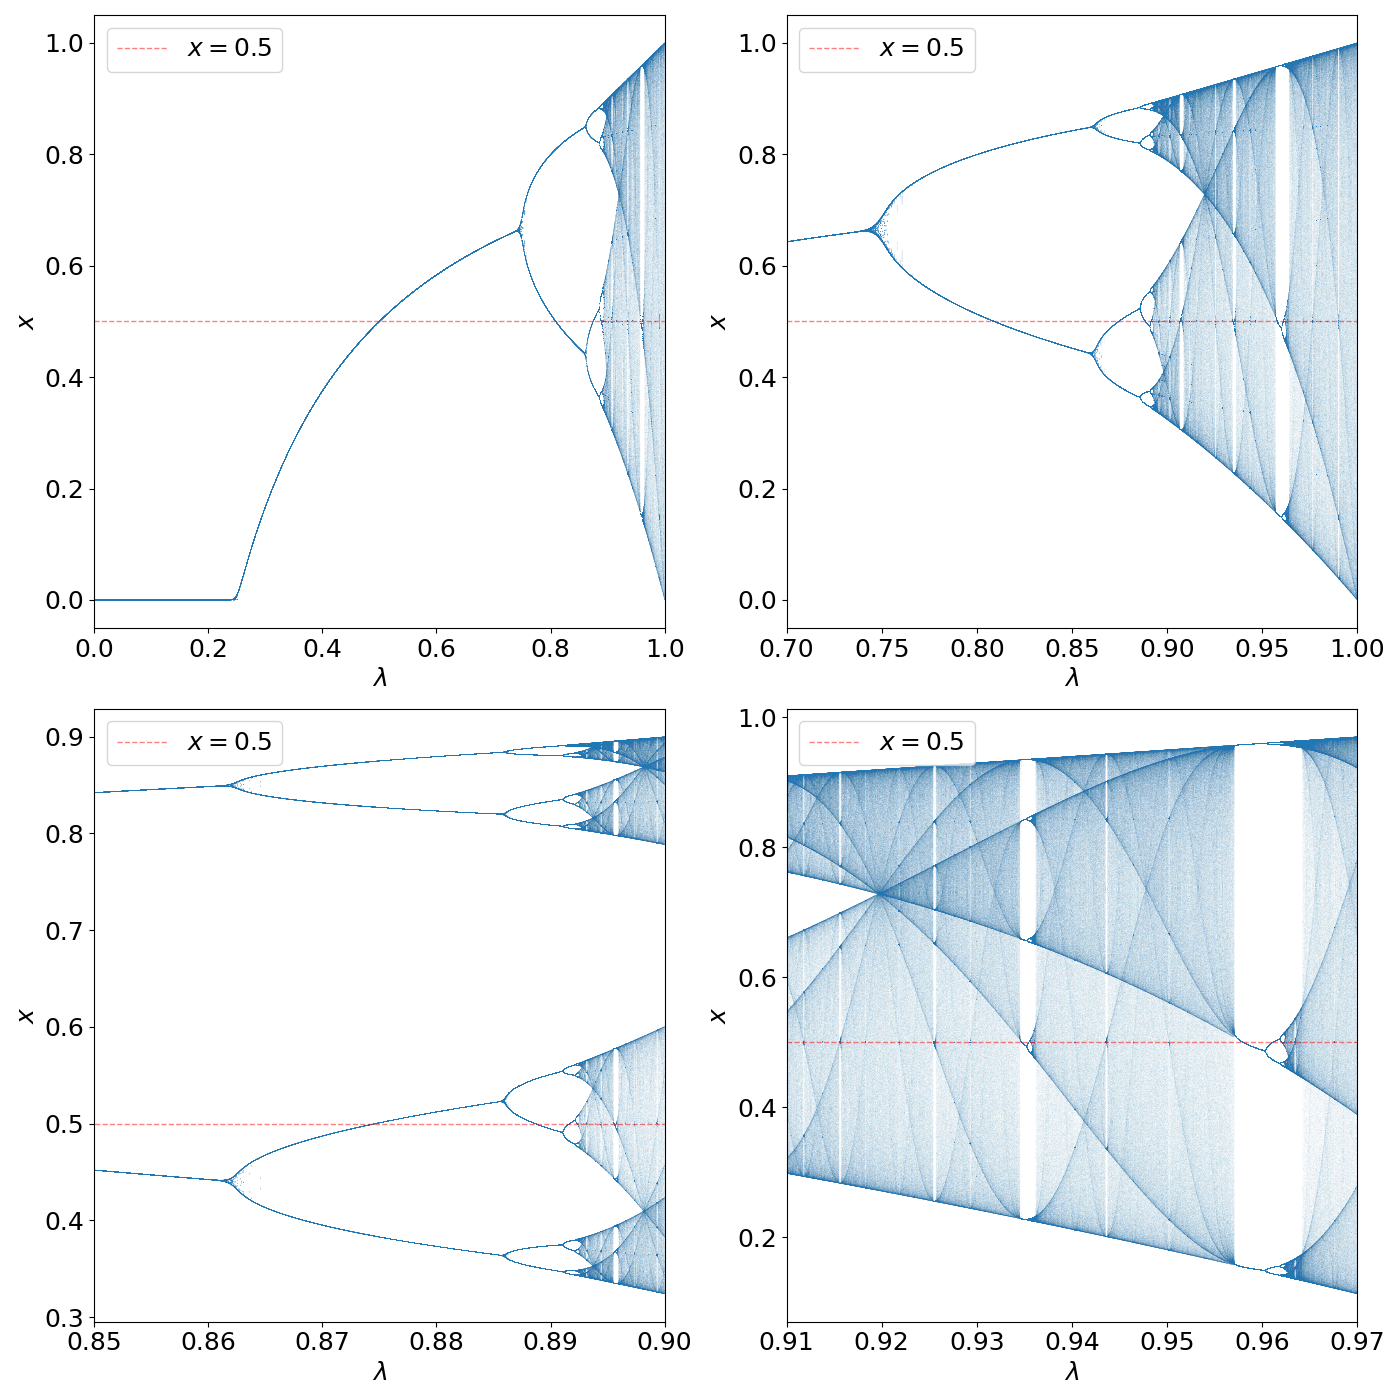
\includegraphics[width=\textwidth]{./figures/logistic.png}
	\caption{
		The graph of logistic bifurcation.
		Each of the subfigures were produced by iterating the logistic map $\L$ with a random starting value $x_0$ to obtain $x_{n+1} = \L(x_n)$ etc., discarding the first several hundred values, and graphing each of the subsequent values as a faint, semi-transparent blue dot at the coordinate $(x, \lambda)$.
		The graph on upper left is the overview of logistic bifurcation on the interval $0 \leq \lambda \leq 1$; upper right and lower right zoomed into the area of periodic doubling, recording $0.7 \leq \lambda \leq 1$ and $0.85 \leq \lambda \leq 0.9$, respectively. Lower right is a zoomed in view of the chaotic region for $ 0.91 \leq \lambda \leq 0.97$. 
	}
	\label{fig:logistic bifurcation overview}
\end{figure}

\begin{observation}[Logistic Bifurcation]\label{th:logistic_bifurcation}
	Let $L_{\lambda} = \lambda 4x(1-x) $ be the logistic function as defined in \eqref{eq_logistic}.
	The dynamical system in a discrete time interval generated by the iteration of the logistic map has the following properties.

	\begin{enumerate}
		\item For $0 < \lambda < a_0 = \frac{1}{4}$, the system has a unique fixed point at $x = 0$. \label{log_fix_0}

		\item For $a_0 <\lambda < a_1 = \frac{3}{4}$, the fixed point at $x=0$ is no longer stable, but a new stable non-zero fixed point emerges. \label{log_fix_1}

		\item When $\lambda$ becomes greater than some value $a_2$, the one cycle becomes unstable, and a stable two cycle appears. 
		Similarly, the 2 cycle will bifurcate into a 4 cycle at $a_3$, $2^n$ cycle to $2^{n+1}$ cycle etc. until $\lambda \rightarrow a_{\infty}$. 
		\label{log_periodic_doubling}
		\item Specifically, for any $\lambda$ there is at most one set of stable orbits. \label{log_at_most_one_stable_orbit}

		\item \label{log_simul_stable_or_unstable}
		Assume for certain $\lambda$ there is an $n$ cycle. That is, there exists distinct $x_1, \cdots, x_n$ such that $\L(x_1) = \L(x_2), \L(x_2) = \L(x_3), \cdots, \L(x_n) = \L(x_1)$.
		Necessarily $x_1, \cdots, x_n$ are $n$ fixed points of $\L^n$. 
		These $n$ distinct fixed point for $\L^n$ must be simultaneously attracting fixed points or repelling fixed points for a given $\lambda$, possibly except for a set of measure zero.

		\item \label{log_cross_half} 
		Let $[a, b]$ be a window of stable orbit of period $n$.
		There exists $\epsilon \in [a, b]$ such that $L_{\epsilon}^n(0.5) = 0.5$. 
		This is the intuitive observation that every orbit must cross the line $x = 0.5$, as shown in the zoomed in view of the bifurcation in figure \ref{fig:logistic bifurcation overview}.

		\item \label{log_closest_branch}
		Observing Figure \ref{fig:logistic bifurcation overview} of the bifurcation pattern in a windows of $2^n$ stable orbits. 
		The previous observation states that there exists a certain $\lambda$ such that $0.5$ is part of the stable orbit, that is $L_{\lambda}^{2^n}(0.5) = 0.5$.
		There is another orbit closest to $0.5$, which spawned from the same bifurcation point.
		The value of this point is $\L^{2^{n-1}}(0.5)$.


		\item  \label{log_chaos_at_1}
			When $\lambda = 1$, the map exhibits chaotic behaviour, defined in Definition \ref{def:Devaney_definition_for_chaos}. 
	\end{enumerate}
\end{observation}

\begin{figure}[htbp]
	\centering
	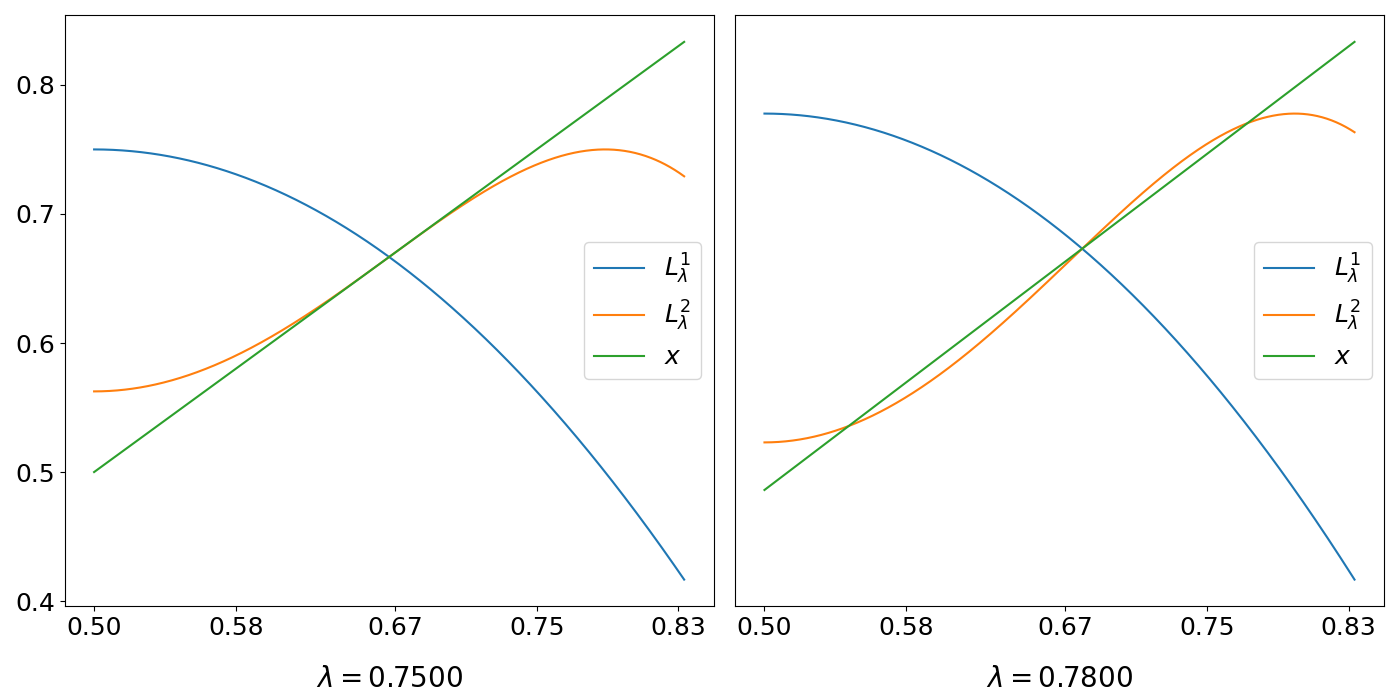
\includegraphics[width=0.8\textwidth]{./figures/logistic_map_around_bifurcation.png}
	\caption{
		$\L, \L^2$ and the function $y=x$ are graphed and zoomed in around the fixed point for $\lambda = 0.75$ and $\lambda = 0.78$, where the bifurcation takes place.
		For $\lambda < 0.75$, as can be seen from Figure \ref{fig:logistic_map_diff_lambda}, the system as a unique stable point. This point loses its stability and a stable two-cycle appears just after $\lambda$ increases above $0.75$.
		This is because, as shown on the right, precisely when the stable fixed point became unstable, the graph of $\L^2$ will have two more intersection with the line $y=x$, which becomes the stable two orbit.
	}
	\label{fig:point_of_bifurcation1}
\end{figure}

\begin{figure}[htbp]
	\centering
	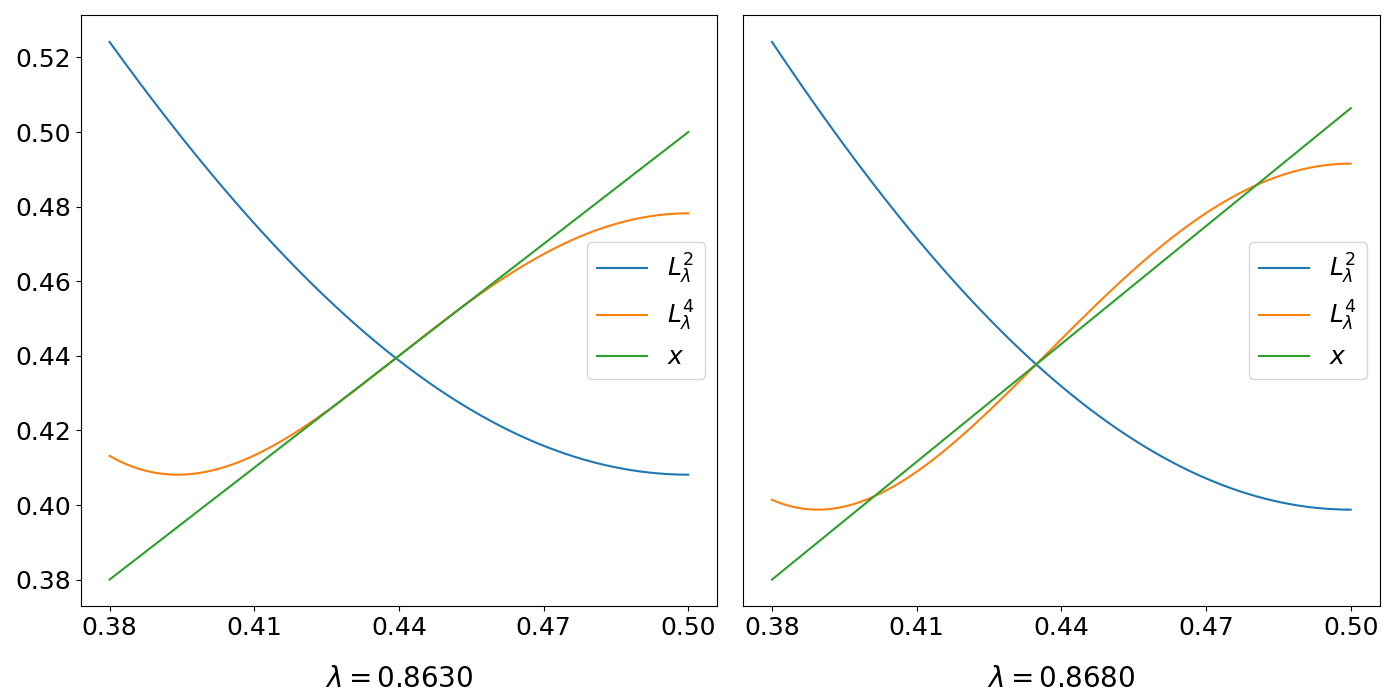
\includegraphics[width=0.8\textwidth]{./figures/logistic_map_around_bifurcation_2.png}
	\caption{Showing $\L^2, \L^4$ and $y=x$ close to one point of second bifurcation similar to Figure \ref{fig:point_of_bifurcation1}}.
	\label{fig:point_of_bifurcation2}
\end{figure}

\begin{proof}[Proof of \ref{th:logistic_bifurcation}.\ref{log_fix_0} and \ref{th:logistic_bifurcation}.\ref{log_fix_1}]
	The fixed point for $\L(x)$ is exactly the solution of the equation $\L(x) = x$, which are $x_0 = 0$ and $x_1 = 1 - \frac{1}{4\lambda}$. 
	$|L_{\lambda}(x_0) | = 4 \lambda < 1$ for $0 < \lambda < \frac{1}{4}$, so by Theorem \ref{th:_stable_unstable_fixed_point}, $x_0$ is a stable fixed point in this interval.
	The argument for $x_1$ is similar.
\end{proof}

% TODO: This prove needs improvements
\begin{proof}[Demonstration of \ref{th:logistic_bifurcation}.\ref{log_periodic_doubling}]
	The proof of this phenomenon again exploits Theorem \ref{th:_stable_unstable_fixed_point}.

	Let us concentrate on $\lambda^*$ at which the fixed point $a$ becomes unstable; that is, $L_{\lambda*}' a  = - 1$ and for any $\lambda > \lambda^*$, the derivative at the fixed point is smaller than $-1$, thus $a$ becomes an unstable fixed point. (This observation is made obvious in Figure \ref{fig:point_of_bifurcation1}.)
	Necessarily, $\frac{d}{dx}L_{\lambda^*}^2 a = L'_{\lambda^*}(a) \cdot L'_{\lambda^*}(a) = 1$,
	and for any $\lambda > \lambda^*$, $\frac{d}{dx}L_{\lambda}^2a'> 1$, where $a'$ is the new fixed point.

	Since $\frac{d}{dx}L_{\lambda}^2(a') > 1$, by mean value theorem for some $\delta > 0$, $\L^2(a' - \delta) < a' - \delta$, and $\L^2(a' + \delta) > a' + \delta$. 
	Observe that $\L^2(1) = 0 < 1$, so by intermediate value theorem there must be some point $b > a' + \delta$ such that $\L^2(b) = b$. 
	Around $a'$ $L^2$ is concaving upwards, meaning its derivative is decreasing, this means that $\frac{d}{dx }L_{\lambda}^2(b) < 1$,
	and we can pick some $\lambda$  close to $\lambda ^*$ such that $-1<\frac{d}{dx }L_{\lambda}^2(b) < 1$, and at this point $b$ is a stable fixed point of $L_{\lambda}^2$.
	The argument for the other fixed point smaller than $a'$ is similar. 

	One significant observation is that the flip of sign of the derivative at the point of bifurcations. 
	To put it precise, at $0.75$ when the fixed point $a$ of $\L^1$ about to lose its stabilitym $\frac{d}{dx} \L(a) = - 1$, and the new fixed point $a'$ of $\L^2$ has $\frac{d}{dx} \L^2(a^*) = 1$. 
	As $\lambda$ increases, the derivative of $\L^2$ at $a^*$ will decrease, and at $a_2$ it will surpass $-1$ and become unstable, and the derivative of the new fixed point of $\L^4$ will be $1$, which will again decrease as $\lambda$ increases.
	This process continues indefinitely.

	All of our arguments above are qualitative, involving only the signs of the derivative and second derivative. 
	Restricting our attention to a neighbourhood of $L^2$ around the point of second bifurcations, all of the above arguments can be applied to $L^2$ and $L^4$. 
	This is the intuition why the bifurcation would continue indefinitely.
	
	The above statement can be made precise and rigourous by the use of Schwarzian derivative, as shown in chapter 12 of \cite{Devaney_green_book_chaos_definition}.
	\footnote{
		The Schwarzian derivative of a function $f$ as $x$ is 
		$$
		Sf(x) = \frac{f'''(x)}{f'(x)} - \frac{3}{2} \left(\frac{f''(x)}{f'(x)}\right)^2.
		$$
		The details derivations of Schwarzian derivative and its application is beyond the scope of this report. 
		Here some of the most fundamental properties are listed.
		\begin{enumerate}
			\item A polynomial $p(x)$ all of whose roots are real and distinct has negative Schwarzian derivative.
			\item If $Sf < 0, Sg < 0$, then $S(f\circ g) < 0$.
			\item If $Sf <0$, $f$ can not have a positive local minimum or negative local maximum.
			\item If $Sf < 0$ and $f$ has finitely many critical points, then $f$ has finitely many attracting points of period $n$ for each $n$.
		\end{enumerate}
	}
\end{proof}

\begin{proof}[Demonstration of \ref{th:logistic_bifurcation}.\ref{log_at_most_one_stable_orbit}]
	This follows from the previous point, but also stems from the fact that $\L^n$ is a function of negative Schwarzian derivative with bounded interval for stable points.
	The number of stable orbits of such maps must not exceed the number of critical points.

	This fact is proved in \cite{Pierre_Collet} and in chapter 11 of \cite{Devaney_green_book_chaos_definition}.
\end{proof}


\begin{proof}[Proof of \ref{th:logistic_bifurcation}.\ref{log_simul_stable_or_unstable}]
		Assuming there exists distinct $x_1, \cdots, x_n$ such that $\L(x_1) = \L(x_2), \L(x_2) = \L(x_3), \cdots $, and $\L(x_n) = \L(x_1)$.

		Differentiate $\L^n$ and evalute at $x_1$ 
		$$
		\frac{d}{dx} \L^n(x_1) = \prod_{i=1}^n \L'(x_i)
		$$

		Indeed evaluting at any other $x_i$ gives the same value. 
		So except for a set of $\lambda$ such that $\frac{d}{dx} \L^n(x_1) = \pm 1$, these $n$ points regarding as fixed points of $\L^n$ must be simultaneously attracting or repelling fixed points by Theorem \ref{th:_stable_unstable_fixed_point}.
\end{proof}

\begin{proof}[Proof of \ref{th:logistic_bifurcation}.\ref{log_cross_half}]
	As shown in the proof of \ref{th:logistic_bifurcation}.\ref{log_simul_stable_or_unstable}, for an $2^n$ cycle of $x_1, x_2, \cdots, x_{2^n}$, differentiate $\L^{2^n}$ and evaluate at any of $x_i$ gives the same value
	$$
	\frac{d}{dx} \L^{2^n}(x) = \prod_{i=1}^{2^n} \L'(x_i)
	$$
	
	In the proof of \ref{th:logistic_bifurcation}.\ref{log_periodic_doubling} we have shown that in a window of stable $2^n$ orbit, the $\frac{d}{dx} \L^{2^n}$ decreases from $1$ to $-1$ as $\lambda$ increase.
	We may assume the derivative at the fixed point is a continuous function of $\lambda$, so by intermediate value theorem there must be some $\lambda$ such that the derivative is $0$. 
	As the derivative equals to the finite product $\prod_{i=1}^{2^n} \L'(x_i)$, one of the $\L'(x_i)$ must be $0$.
	Logistic map has a unique maximum $0.5$, and this will take place iff one of the $x_i = 0.5$.
\end{proof}

\begin{proof}[Demonstration of \ref{th:logistic_bifurcation}.\ref{log_closest_branch}]
	Assuming $a_0$ is one of the points in a stable $2^{n-1}$ orbits, then $\L^{2^{n-1}}(a_0)=a_0$ for $\lambda$ in its window.
	As $\L(x)$ is a continuous function of both $x$ and $\lambda$, small perturbations of $\lambda$ will result in small perturbations of $\L^{2^{n-1}}(a_0)$, so, after $\lambda$ increase beyond the window for $2^{n-1}$ orbit and $\L^{2^{n-1}}(a_0) \neq a_0$, but its value shall still stay close to $a_0$.
\end{proof}


\begin{proof}[Proof of \ref{th:logistic_bifurcation}.\ref{log_chaos_at_1}]
	The doubling map \eqref{eq:doubling_map}, which is chaotic, is topologically conjugate to $L_{\lambda}$, where $\lambda = 1$, so $L_{\lambda}$ is chaotic.
	This is proved in Example \ref{ex_logistic_and_doubling}.
\end{proof}

\section{Feigenbaum's Constants}

Another striking observation from Figure \ref{fig:logistic bifurcation overview} is that the overall shape of the graph exhibits some kind of fractal structure that is \emph{self similar}.
If only focusing on one branch of bifurcation and disregarding the coordinates, the shape of each bifurcation is similar to any other up to elongation and stretching, including the branches bifurcated out from itself.
 
 This observation is crucial to many properties of iterated maps and leads naturally to the conjecture that each bifurcation is scaled down from its parent, and there are some constants to describe the ratio of the scaling. 

 There are two ways to quantify this self-similarity: the spacing between each bifurcation points, and the distance between the superstability point and the point closest to it in the stable orbit. 
 In either case we can compute numerically the values of $x$ and $\lambda$.

 Numerical computation of the bifurcation point beyond the first few terms is difficult, as near the bifurcation points the iterated maps converge very slowly.
 Instead, we can compute the point of superstability where the rate of the convergence is fastest by using Theorem \ref{th:logistic_bifurcation}.\ref{log_cross_half}, which states that each of the stable orbits must cross $0.5$ where they achieve superstability ($\frac{d}{dx}\L^{2^n}(0.5) = 0$).
In this report we will label the value of $\lambda$ as $A_n$ at which the superstability point of $2^n$ cycle is attained.
Once $A_n$ are known, Theorem \ref{th:logistic_bifurcation}.\ref{log_closest_branch} states that the coordinate of the point in the bifurcation cycle closest to $0.5$ (which is also part of the bifurcation cycle as super-stability is attained) is $\L^{2^{n-1}}(0.5)$. (Recall at $A_n$ there a stable $2^n$ cycle emerges.)
Therefore the distances between them is $|\L^{2^{n-1}}(0.5) - 0.5|$ and are labelled as $d_n$.
Figure \ref{fig:demonstration of feigenbaum constants on logistic map} is a demonstration of $A_i$ and $d_i$ on logistic map.

The values of $A_n$ and $d_n$ calculated numerically are shown in Table \ref{tab:feigenbuam_alpha_table_for_logistic}. 
The observation is clear:
$\frac{A_{n+1}-A_n}{A_{n+2}-A_{n+1}}$ approaches approximately $4.668$ as $n \rightarrow \infty$, and $\frac{d_n}{d_{n+1}}$ approaches approximately $2.503$ as $n \rightarrow \infty$. 
The former is known as Feigenbaum's constant $\delta \approx 4.6692016091023$, the latter Feigenbaum's constant $\alpha \approx 2.5029078750957$ \cite{F1}.
The reason these constants are worth such as denominations is that they are \emph{universal}.

\begin{table}
\centering
\begin{tabular}{|c|c|c|c|c|}
\hline
\( n \) & \( A_n \) & \( d_n \)  & \(\frac{A_{n+1} - A_n}{A_{n+2} - A_{n+1}}\)  &  \(\frac{d_n}{d_{n+1}}\) \\ \hline
0 & 0.5000000000 & - & 4.5358092997 & - \\
1 & 0.8064950000 & 0.3064950000 & 4.6838460230 & 2.6616365278 \\
2 & 0.8740672853 & 0.1151528380 & 4.6103617168 & 2.5423697165 \\
3 & 0.8884939520 & 0.0452935060 & 4.6110890246 & 2.5175763063 \\
4 & 0.8916231352 & 0.0179909169 & 4.6981361800 & 2.5029942863 \\
5 & 0.8923017565 & 0.0071877579 & 4.5692030565 & 2.5187506567 \\
6 & 0.8924462013 & 0.0028536996 & 4.6976886127 & 2.5019617749 \\
7 & 0.8924778140 & 0.0011405848 & 4.5707037850 & 2.5191930664 \\
8 & 0.8924845434 & 0.0004527580 & 4.6690000000 & 2.5048153706 \\
9 & 0.8924860157 & 0.0001807550 & 4.6410832897 & 2.5116759261 \\
10 & 0.8924863310 & 0.0000719659 & 4.5599414736 & 2.5226365150 \\
11 & 0.8924863990 & 0.0000285281 & 4.6418936559 & 2.5096745464 \\
12 & 0.8924864139 & 0.0000113672 & 4.6286915064 & 2.5130534587 \\
13 & 0.8924864171 & 0.0000045233 & 4.6027721102 & 2.5181104605 \\
14 & 0.8924864178 & 0.0000017963 &  - & 2.5201147995 \\
15 & 0.8924864179 & 0.0000007128 &  - &  - \\
\hline
\end{tabular}
\caption{
	Values of \( A_n \), \( \delta_n \), and their ratios for the logistic map.
	Each $a_n$ is the value of $\lambda$ such that $\L^{2^n}(0.5) = 0.5$, which is the value of $\lambda$ where the $2^n$ cycle crossed the $y=0.5$ line. 
	Each $\delta_n$ is the difference between between 0.5 and the closest point in the $2^n$ cycle at $A_n$.
	The ratios of there difference are also calculated.
}
\label{tab:feigenbuam_alpha_table_for_logistic}
\end{table}

\begin{figure}
	\centering
	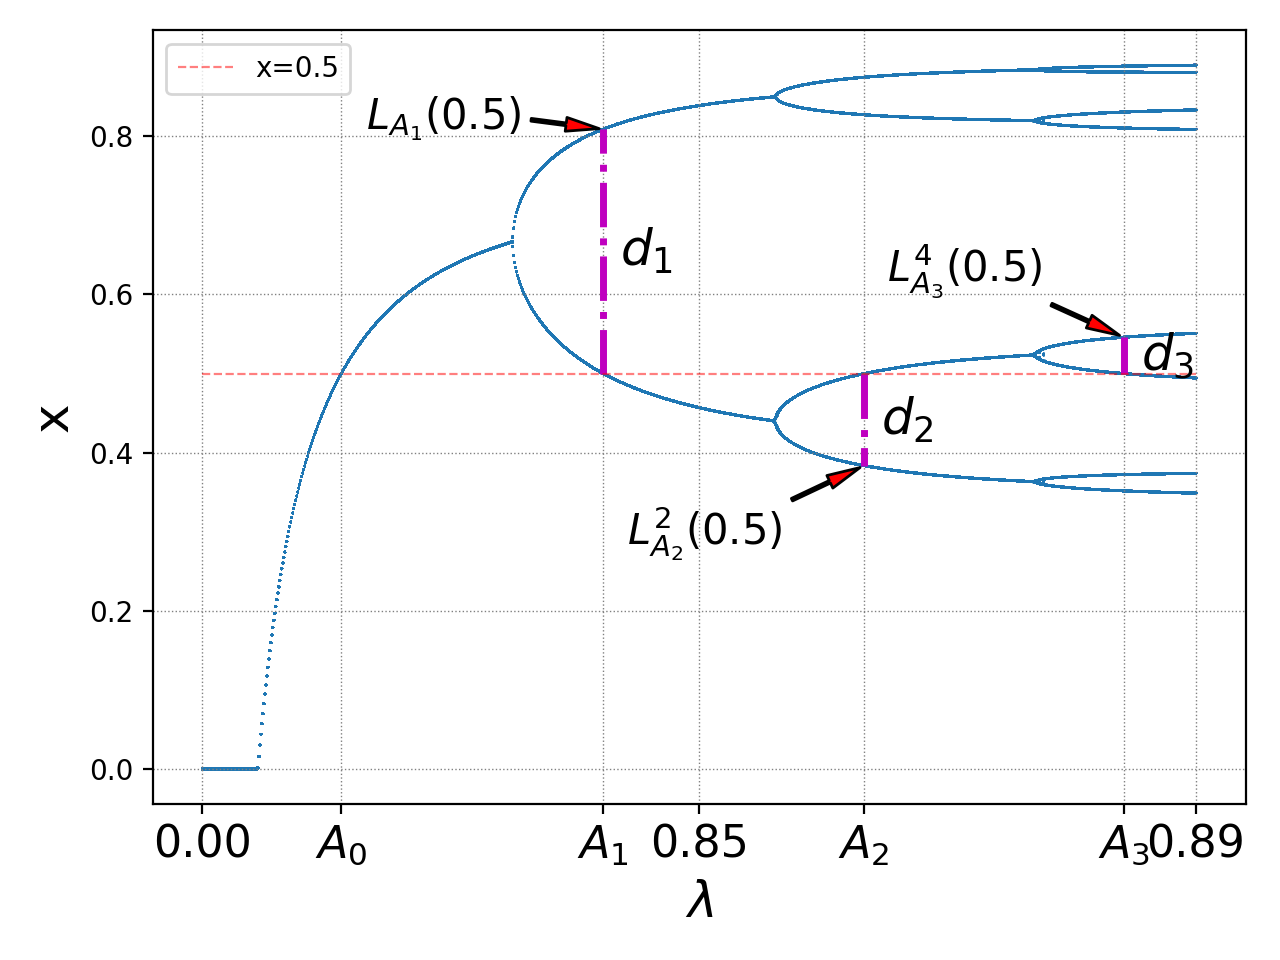
\includegraphics[width=0.8\textwidth]{./figures/demonstration of feigenbaum constants.png}
	\caption{ 
		A portion of the bifurcation diagram of the logistic map with demonstration of  $A_i$, which is the value of $\lambda$ at which the superstability of $2^i$ cycle is attained, and $d_i$, which is the distance between the superstability point (at $x=0.5$) and the closest point in the stable orbit.
		The $\lambda$ axis in in logarithmic scale, and the transformation to from $\lambda$ to $x$ coordinate is $-\log(A_{\infty} - \lambda)$.
	}
	\label{fig:demonstration of feigenbaum constants on logistic map}
\end{figure}

It is worthwhile to describe our algorithm to compute $A_i$ and $d_i$ in detail, as such seemingly innocuous computation is actually surprisingly challenging.
As for as the authors' knowledge, computations of $A_i$ to such precision has not been performed previously, and the method described here is original.

The first challenge is the precision of floating point arithmetic.
At $n = 10$, the value of $A_{n+1} -A_{n} $ is smaller than $ 10^{-8}$. 
To compute $\frac{A_{n+1} - A_n}{A_{n+2} - A_{n+1}}$ to $8$ significant figures (base 10), therefore, would require calculating $A_i$ to 16 significant figures, greater than the precision of the double precision floating point used in most computers, which only allows approximately 15 significant figures
\footnote{
	The IEEE standard for floating point arithmetic \cite{IEEE_floating_point} (IEEE 754) decrees 53 bits of binary digits in double precision floating point (page 8, table 3.2 of the standard.) This translates to $53 \cdot \log_{10}(2) \approx 15.8$ significant digits based 10.
}.
The only way to overcome this is to use an arbitrary precision arithmetic library. 
We chose to use GNU GMP (GNU Multiple Precision Arithmetic Library) \cite{GMP} with interface in C++.

The next challenge is the efficiency of the algorithm. 
If the algorithm starts by trying each $\lambda = 0$ and increments by $10^{-8}$ until $\lambda$ reaches $1$, the computer needs to compute literally billions of iterations of the logistic map, taking very long time and much wasted computer power.
The natural optimisation is to guess approximately where $A_i$ shall be and check $\lambda$ with greater precision in that area. 
In the process of guessing we still need to increment $\lambda$ by some difference, but initial increment of $\lambda$ can be relatively large, and whenever a value of $A_i$ is found, this difference shall be scaled down by Feigenbaum's  $\delta$.


While the full code in C++ was included in the appendix,
Algorithm \ref{ag:compute A_i} shows the pseudocode, which needs input parameters $\lambda_{start}$ for the start of $\lambda$, $\lambda_d$ for the initial increment of $\lambda$, and $n_{bound}$ for the maximum number of $A_i$ to be computed.
Algorithm \ref{ag:compute A_i} depends on Algorithms \ref{ag:super stable} and \ref{ag:fine tuning}. 
The former checks if superstability under a threshold is obtained at a certain $\lambda$, and the latter fine tunes $\lambda$ to obtain the most accurate value of $A_i$.
Both algorithms require various parameters including the threshold for superstability and the constant $c$ for fine tuning.
By poking different values for parameters of this algorithm, reasonably accurate numerics can be obtained up to $A_{15}$.


\begin{algorithm}
	\caption{Check if $\lambda$ is super stable}
	\begin{algorithmic}[1]
		\Require $\lambda$, cycle number $n,$ point of superstability $x^* = 0.5$, and threshold $t$.
		\If{$|L_{\lambda}^{2^{n-1}}(0.5) - 0.5| < t$}
		\State \Return True
		\Else
		\State \Return False
		\EndIf
	\end{algorithmic}
	\label{ag:super stable}
\end{algorithm}

\begin{algorithm}
	\caption{Fine Tuning $\lambda$}
	\begin{algorithmic}[1]
		\Require $\lambda$, cycle number $n,$ point of superstability $x^* = 0.5$, and an constant $c$. $\lambda \in (\lambda - c, \lambda +c)$ are checked.
		\State Create a list $L$ of $\lambda$ in the interval $I$.
		\State Compute the list $L^*$, which holds $L_{\lambda}^{2^{n-1}}(0.5)$ for each $\lambda$ in $L$.
		\State Set $\lambda$ to be the element in $L$ corresponding to the minimum value in $L^*$.
		\State Perform fine tuning by repeating the above steps after setting $c = c / \delta$. \Comment{$\delta$ is Feigenbaum's delta}
		\State Iteration stops when $c$ is smaller than a certain threshold.
	\end{algorithmic}
	\label{ag:fine tuning}
\end{algorithm}

\begin{algorithm}
	\caption{Computation of $A_i, d_i$}
	\begin{algorithmic}[1]
		\Require $\lambda = \lambda_{start}$, $A_i = \{0.5\}, d_i = \{\}$, and cycle number $n = 2$ (We have computed the first stability point is $0.5$, so we can start with cycle number $2$.)
		\While{$\lambda < \lambda_{end}$ and $len(A_i) < n_{bound} $}
		\If{$L_{\lambda}(0.5)$ is super stable}  \Comment{Using algorithm \ref{ag:super stable}}
			\State Fine tuning $\lambda$ with algorithm \ref{ag:fine tuning}.
			\State Append $\lambda$ to $A_i$ 
			\State Append $\L^{2^{n-1}}(0.5)$ to $d_i$ 
			\State $\lambda = \lambda + \lambda_{i}$
			\State $\lambda_{d} = \lambda_d / \delta$  \Comment{$\delta$ is Feiganbaum's delta}
			\State $\lambda_{i} = \lambda_i / \delta$
			\State $n = n + 1$
		\EndIf
		\State $\lambda = \lambda + \lambda_d$
		\EndWhile
	\end{algorithmic}
	\label{ag:compute A_i}
\end{algorithm}

\section{Single Nodal Functions Give Rise to Bifurcations}

Our previous discussion of infinite bifurcations of the logistic map is qualitative and the proof of Theorem \ref{th:logistic_bifurcation} only relies on the facts that the logistic map is differentiable, concaves downwards, has a unique maximum, and has negative Schwarzian derivative. 
It may not be of surprise, therefore, that the dynamical properties of bifurcation are shared among a large class of functions with very moderate restrictions.
Let us investigate some more examples.

Figure \ref{fig:combined_bifurcations} shows the bifurcation diagrams of $f(\lambda, x) = \lambda \sin(2\pi x)$, $f(\lambda, x) = \lambda + \sin(2\pi x)$, $f(\lambda, x) = \lambda x(1-x)^2$, and $f(\lambda, x) = \lambda x \log(x)$.
Infinite bifurcation and periodic doubling to chaos were observed for all cases, although the exact values of $\lambda$ at which the bifurcation take place is different for each map.
It is also striking that the shape of each bifurcation diagram is extremely similar to that of the logistic map up to elongation and stretching, so it is reasonable to conjecture that most of the points of Theorem \ref{th:logistic_bifurcation} shall also apply to these functions.
Indeed, point \ref{log_cross_half} of Theorem \ref{th:logistic_bifurcation} is readily demonstrated by Figure \ref{fig:combined_bifurcations}
as, in each subfigure, the horizontal line at the local maximum crosses the stable orbits of any periods at some $\lambda$.

% TODO: How shall we name these diagram if there is no bifurcation?
Figure \ref{fig:combined_no_bifurcations} shows the bifurcation (or the lack of bifurcation) diagrams of $\lambda \sin(2\pi x)$, $\lambda + \sin(2\pi x)$, $\lambda x(1-x)^2$, and $\lambda x \log(x)$. 
Each of these functions exhibit dynamical behaviour different from periodic bifurcations.
The $\lambda e^x$ map bifurcated precisely once at $-e$. 
For all $\lambda < -e$ there are two stable orbit, while for $\lambda > -e$ there are one stable orbits.
As for the tent map, there is one unique stable fixed point $x=0$ for $\lambda \in [-0.5, 0.5]$, and for any other $\lambda$ there seems to be no stable orbits at all but homogeneous region of chaos. 
The fact that tent map is chaotic is proved in Example \ref{ex:logistic and tent}.
The two $\arctan$ maps have similar behaviours to the exponential map. 
Their stable orbit only bifurcated once over all $\lambda \in \bb{R}$.

Why do the former class of functions exhibit infinite bifurcations to chaos, but the latter class do not?
The graphs of these functions, shown in Figure \ref{fig:combined_bifurcations_functions_graph}, may give the answer. 
All functions which give rise to bifurcations are smooth and have single-modal structures; that is, their values are bounded and attain unique maximums in some interval. Those which do not exhibit bifurcation are either not differentiable at the maximum, e.g. the tent map, or do not have local maxima, e.g. the exponential and arctangent maps.
This observation fits our expectation, as in the proof of Theorem \ref{th:logistic_bifurcation}, the most important property used is the fact that the logistic function attains a unique, differentiable maximum at $x=0.5$ and it concaves downwards. 
Metropolis et al. \cite{metropolis2017finite} have shown that the bifurcation phenomenon is universal, as summarised in the following theorem.

\begin{thm}[Criterion for infinite bifurcations]\label{th:criteria_for_infinite_bifurcations}
	If $f(x)$ satisfies the following properties:
	\begin{enumerate}
		\item $f(x)$ is continuous, singled valued, piecewise $C^1$ and has a unique differentiable maximum on the interval $[0,1]$ attained at $x^*$;
		\item $f(x) > 0$ on $(0,1)$, $f(0) = f(1) = 0$, and $f$ is strictly increasing in $[0, x^*]$ and strictly decreasing in $[x^*, 1]$;
		\item for $\Lambda_0 < \lambda < 1, \lambda f(x)$ has two fixed points (one of which is $x = 0$) both of which are repellent, that is $|\lambda f'(x)| > \frac{1}{\lambda}$; and,
		\item in the interval $N$ around the unique maximum $f$ concaves down-wards,
	\end{enumerate}
	then the system $x_{n+1} = \lambda f(x_n)$ will exhibit infinite bifurcations and periodic doubling to chaos.
	To be precise, the criterion for chaos by period doubling bifurcations is:
	\begin{enumerate}
		\item for $\Lambda_0 < \lambda < \lambda_{\infty} < 1$, there exists stable orbit of period $2^n$ for all $n = 1, 2, \cdots$. with $n$ increasing with $\lambda$; and
		\item for each $\lambda$, there exists at most one set of stable orbits.
	\end{enumerate}
\end{thm}

\begin{figure}
	\centering
	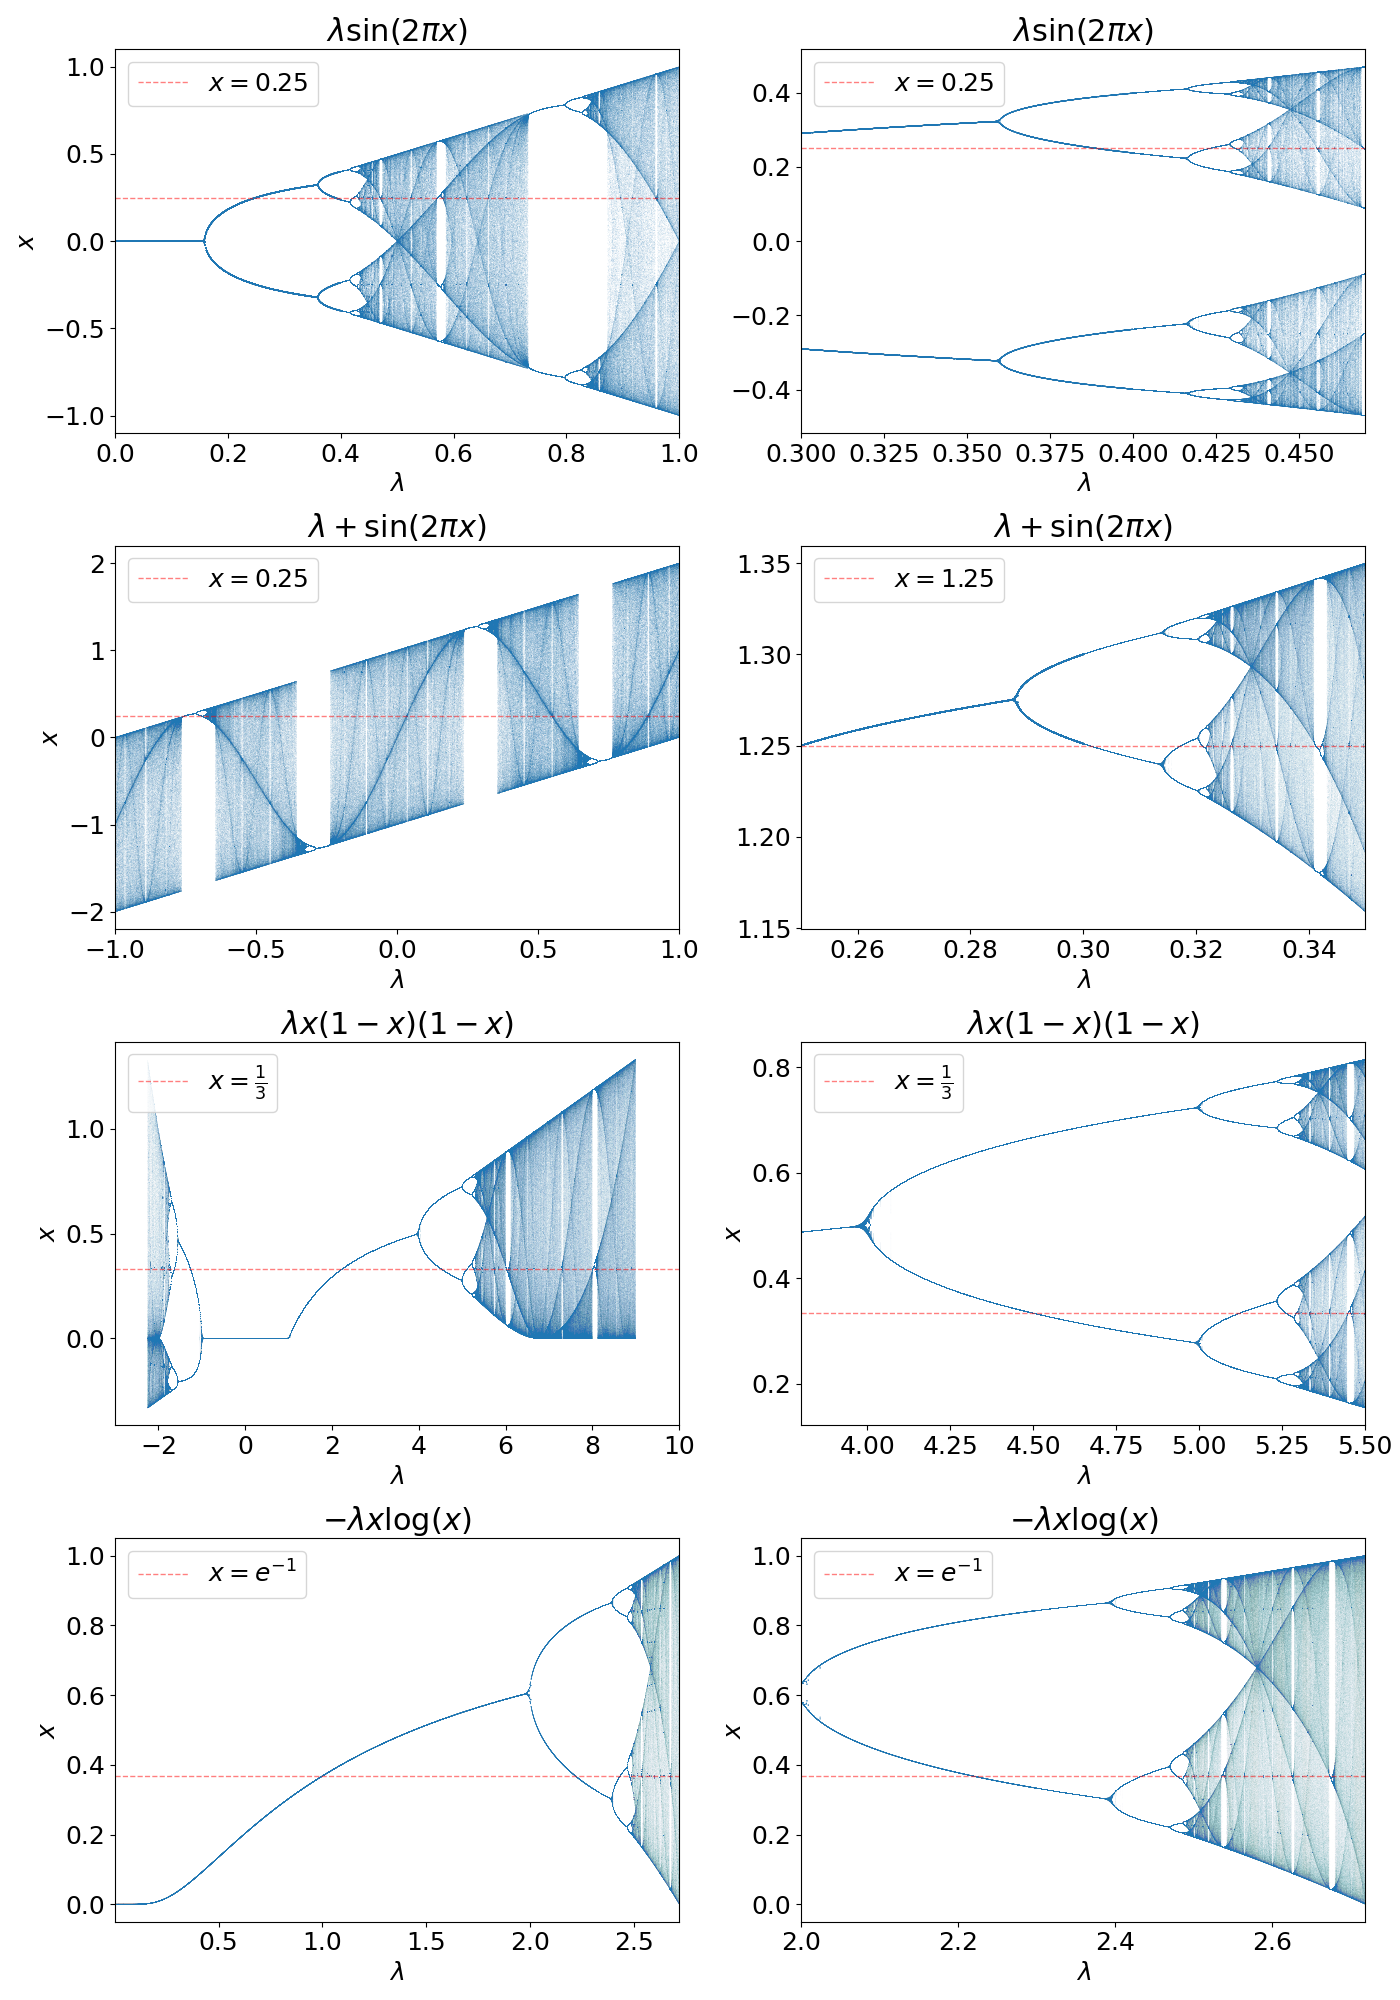
\includegraphics[width=\textwidth]{./figures/combined_bifurcations.png}
	\caption{
		Bifurcations diagrams of four different functions 
		$ \lambda \sin(2\pi x)$,
		$ \lambda + \sin(3\pi x)$,
		$ \lambda x(1-x)^2$,
		and $ \lambda x \log(x)$.
		All of these functions exhibit bifurcations and periodic doubling to chaos like the logistic map. 
		The subfigures on the left are the overview of bifurcations, where the ones on the right are zoomed in around points of bifurcation.
		The graph of these functions are presented in Figure \ref{fig:combined_bifurcations_functions_graph}
	}
	\label{fig:combined_bifurcations}
\end{figure}

\begin{figure}
	\centering
	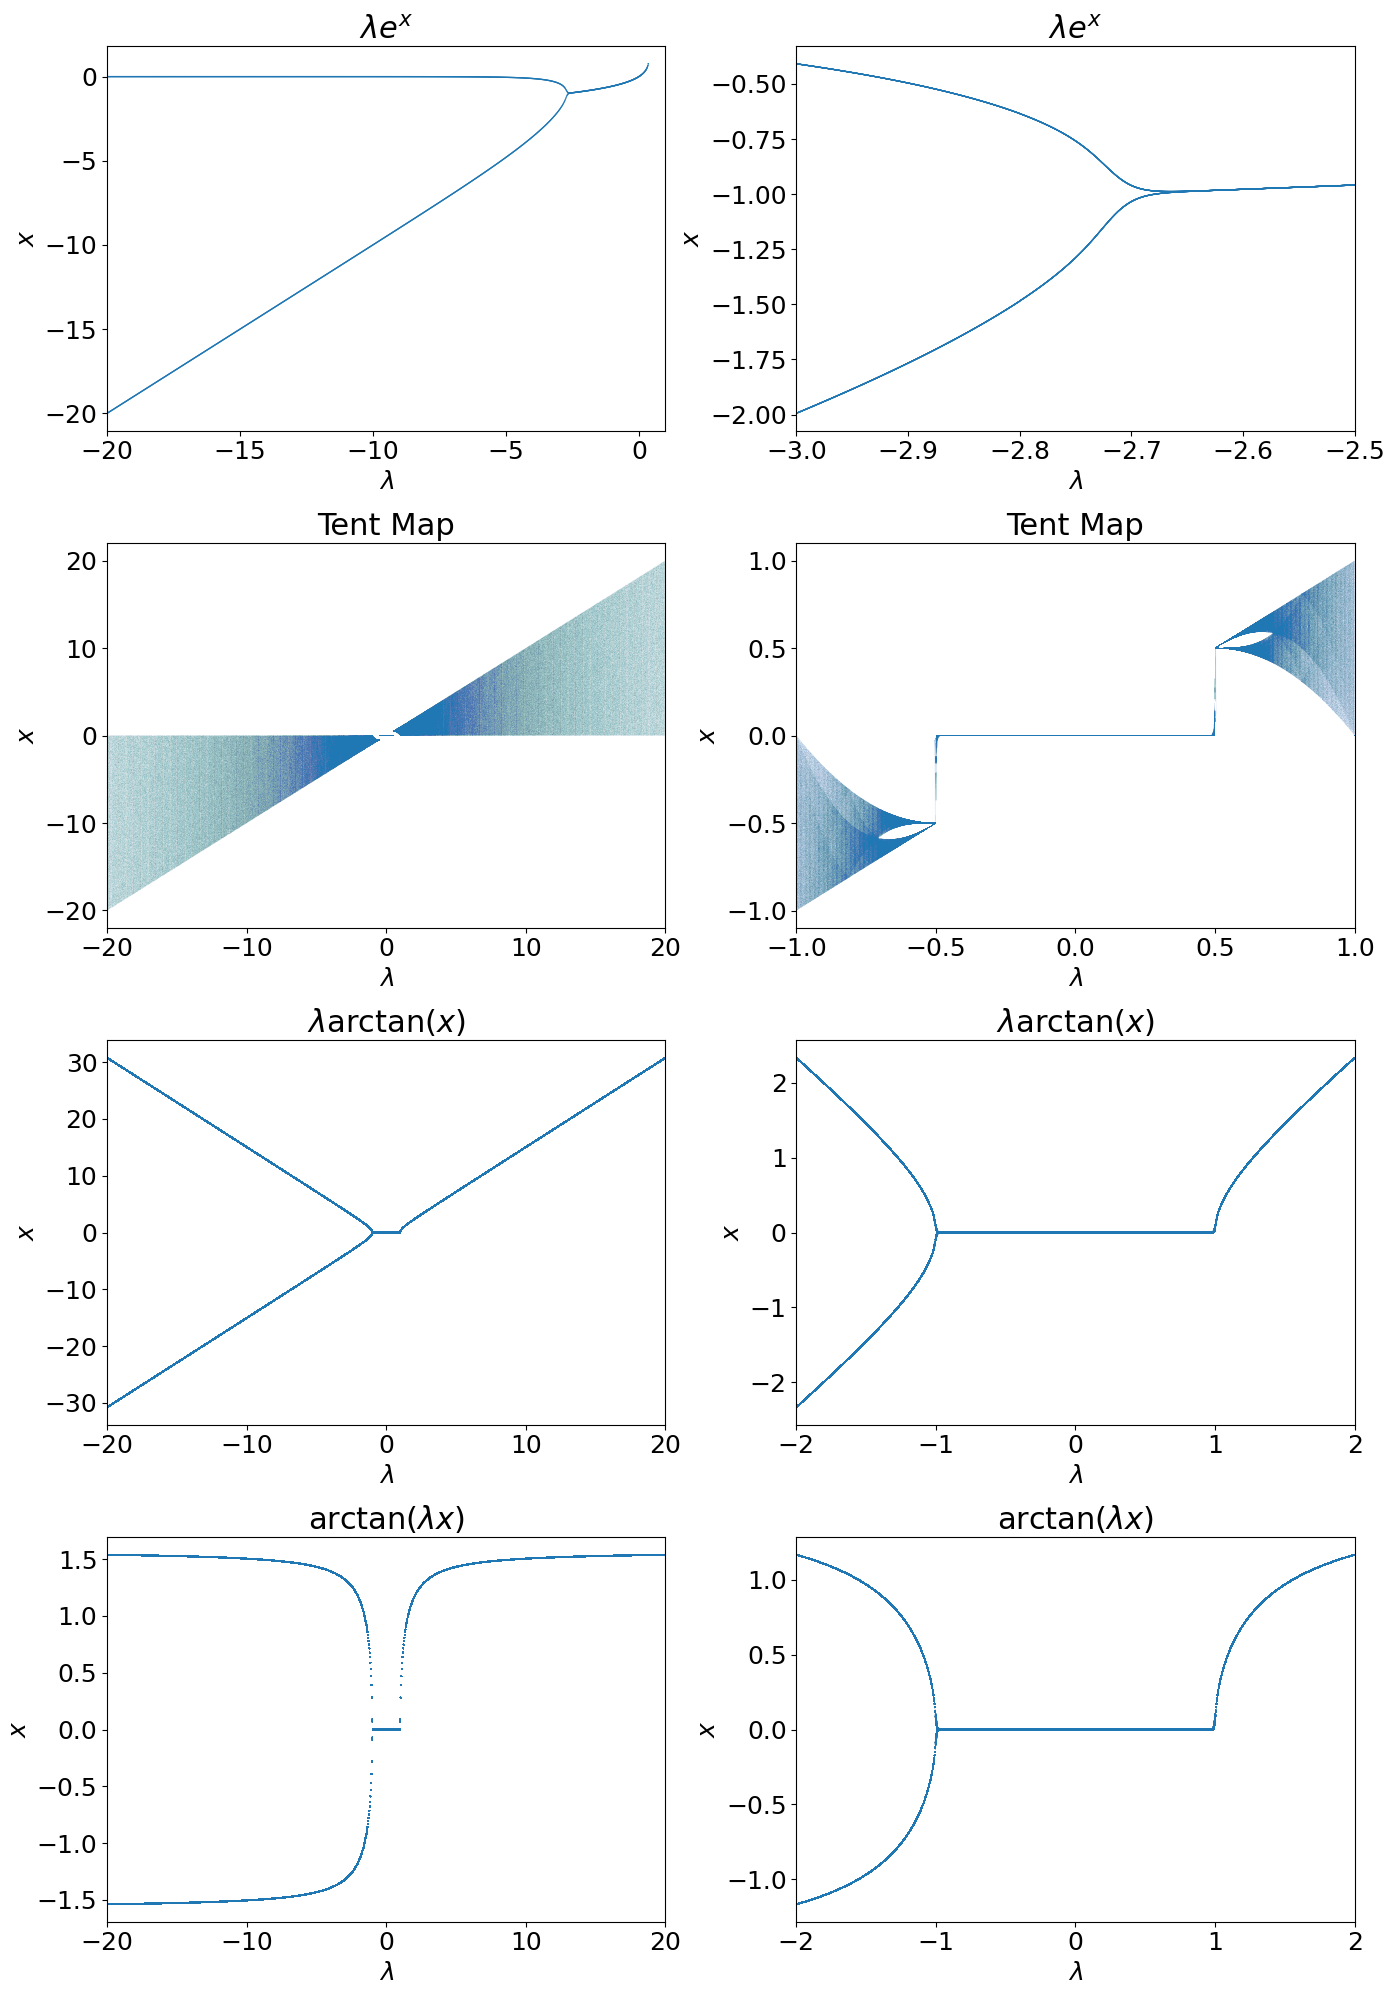
\includegraphics[width=\textwidth]{./figures/combined_no_bifurcations.png}
	\caption{
		These figures show patterns of (or lack of) stable orbits for four functions which do not exhibit periodic doubling to chaos. 
		The graph of these functions were presented in Figure \ref{fig:combined_bifurcations_functions_graph}.
	}
	\label{fig:combined_no_bifurcations}
\end{figure}

\begin{figure}
	\centering
	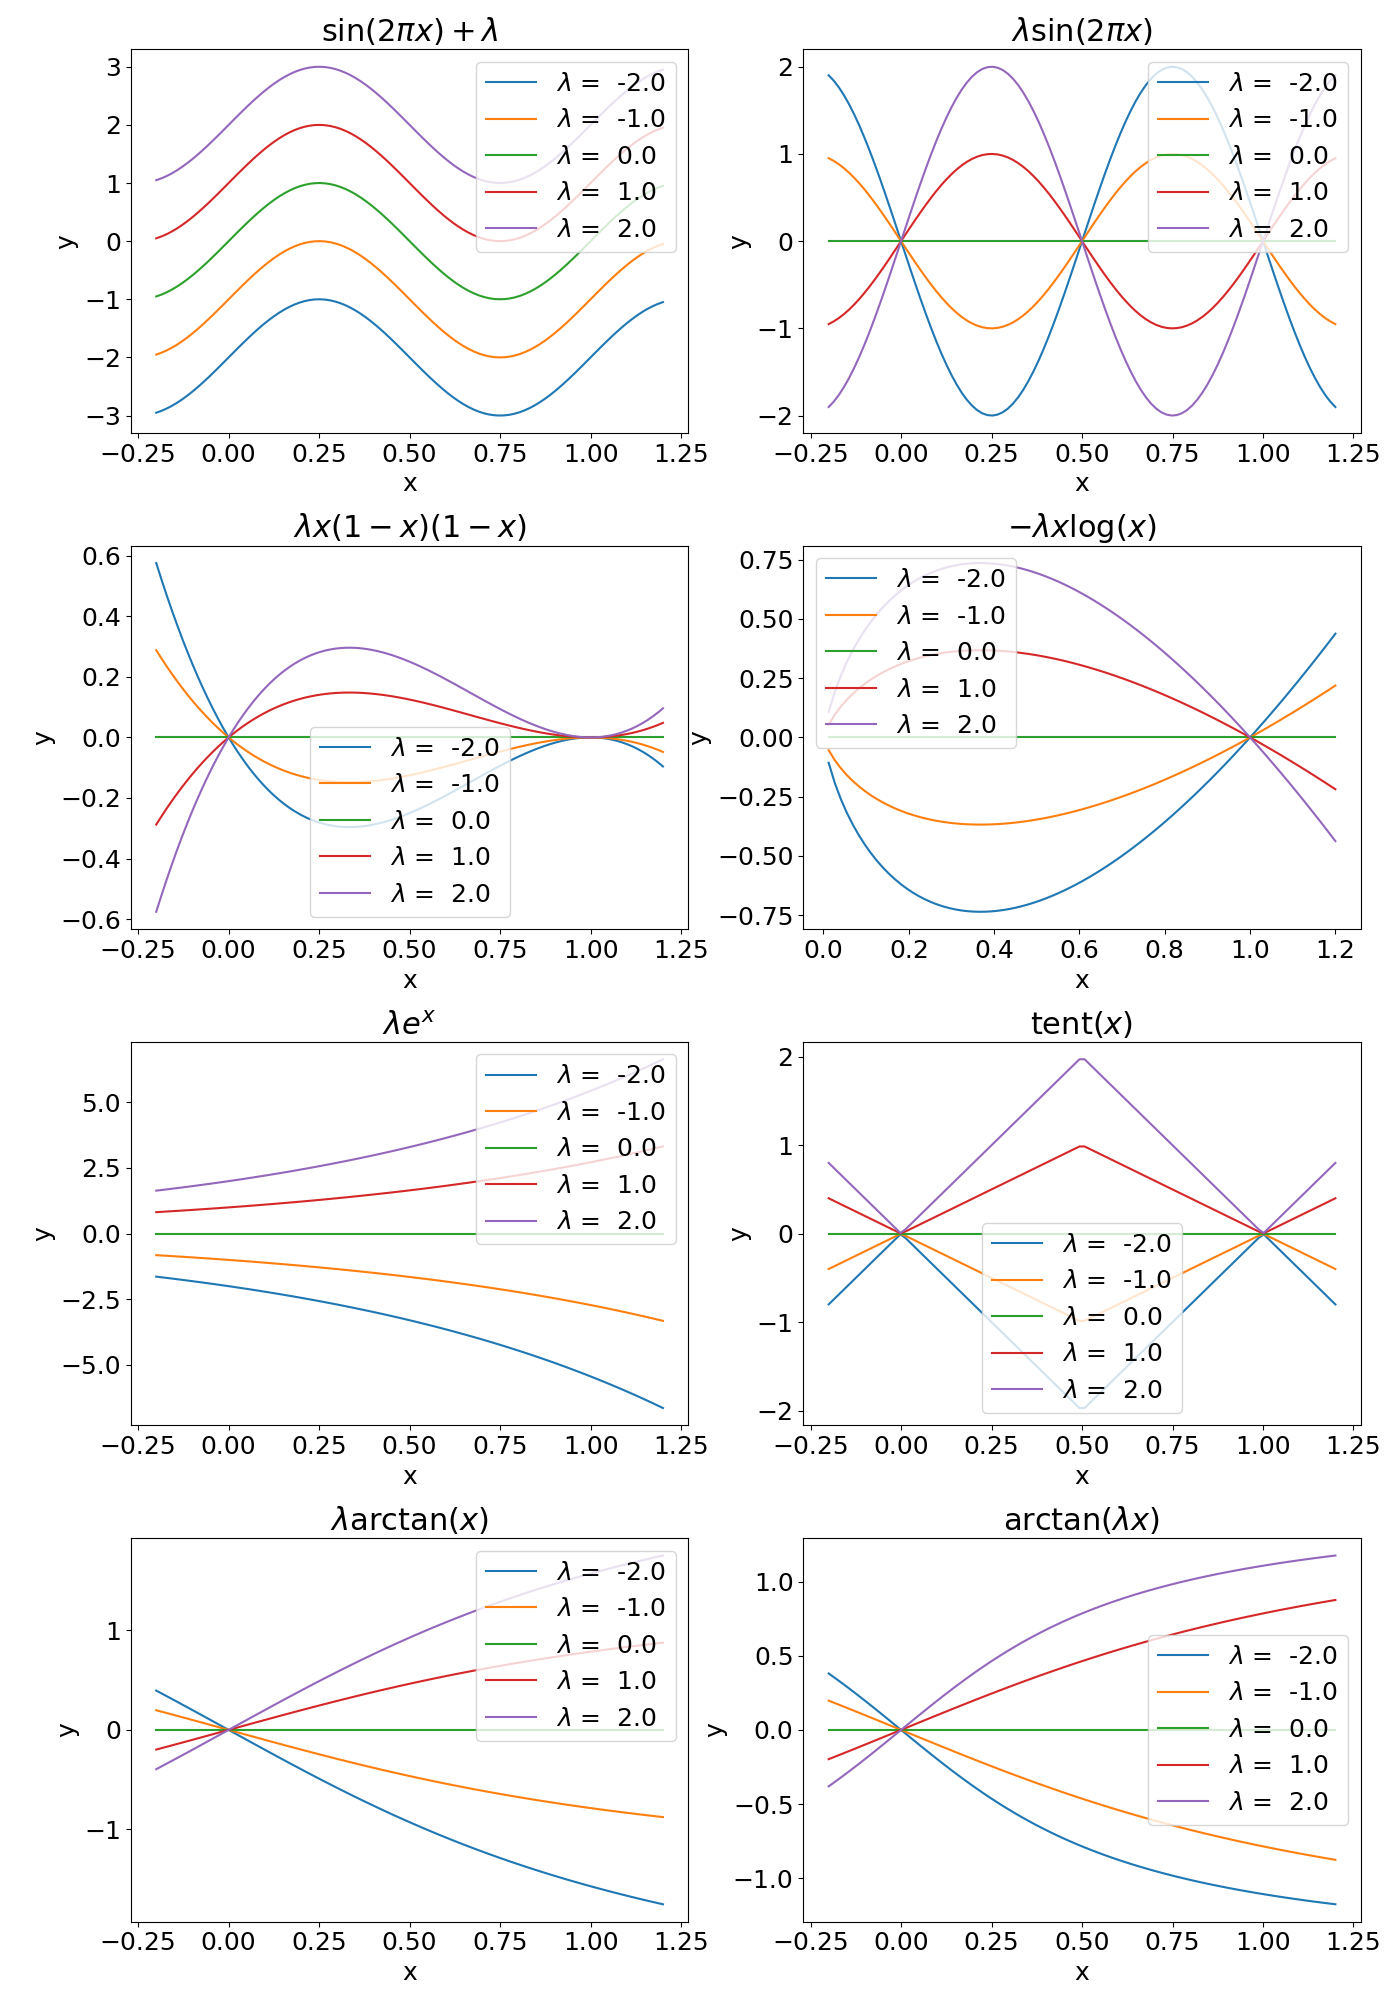
\includegraphics[width=\textwidth]{./figures/combined_functions.png}
	\caption{
		This figure shows the graph of the functions whose bifurcation diagrams are graphed on Figure \ref{fig:combined_bifurcations} and \ref{fig:combined_no_bifurcations}.
	}
	\label{fig:combined_bifurcations_functions_graph}
\end{figure}


Having settled that the periodic bifurcation is a universal phenomenon for a large class of functions, naturally we ask how about the scaling constants shown in Table \ref{tab:feigenbuam_alpha_table_for_logistic}.
The surprising fact is that Feigenbaum's constants $\delta$ and $\alpha$ are universal for any iterative map depending on one variable and exhibit periodic doubling bifurcations with orbit $2^0, 2^1, 2^2, \cdots$. 
Indeed, Tabor showed that such constants are universal for iterative maps with negative Schwarzian derivative \cite{Tabor}.
The entirety of the last chapter will be dedicated to the demonstration of this fact based on Feigenbaum's theory of scaling. 
Here, instead, we present another numerical evidence for the universality of Feigenbaum's constants.

Table \ref{tab:feigenbuam_constants_skewed_logistic_map} shows the $A_i$, $d_i$, and their ratios for the skewed logistic map $f_{\lambda} (x) = \lambda x (1-x)^2$.
The numerics were calculated with an algorithm similar to Algorithm \ref{ag:compute A_i}.
Although the speed of convergence is clearly different, 
$ \frac{d_n}{d_{n+1}} $ and $\frac{A_{n+1} - A_n}{A_{n+2} - A_{n+1}}$ seem to converge to the same number as in the logistic map.
\begin{table}
\centering
\begin{tabular}{|c|c|c|c|c|}
\hline
\( n \) & \( A_n \) & \( d_n \)  & \(\frac{A_{n+1} - A_n}{A_{n+2} - A_{n+1}}\)  &  \(\frac{d_n}{d_{n+1}}\) \\ \hline
0 & 2.25000000 & - & 3.58291025 & - \\
1 & 4.49325749 & 0.33233444 & 4.41239995 & 3.11334650\\
2 & 5.11935677 & 0.10674508 & 4.60351732 & 2.31871272 \\
3 & 5.26125217 & 0.04603635 & 4.65268653 & 2.58607785 \\
4 & 5.29207543 & 0.01780161 & 4.66307535 & 2.47302222 \\
5 & 5.29870026 & 0.00719832 & 4.65793977 & 2.51729830 \\
6 & 5.30012096 & 0.00285954 & 4.67119534 & 2.49830019 \\
7 & 5.30042596 & 0.00114459 & 4.64986027 & 2.50813287 \\
8 & 5.30049126 & 0.00045635 & 4.65947170 & 2.50369628 \\
9 & 5.30050530 & 0.00018227 & 4.66753118 & 2.50386731 \\
10 & 5.30050832 & 0.00007279 & 4.66237768 & 2.50460649 \\
11 & 5.30050896 & 0.00002906 & 4.64855560 & 2.50672818 \\
12 & 5.30050910 & 0.00001159 & 4.65083889 & 2.50600317 \\
13 & 5.30050913 & 0.00000462 & 4.66534446 & 2.50451859 \\
14 & 5.30050914 & 0.00000184 &  - & 2.50767228   \\
15 & 5.30050914 &  0.00000073&  - &  - \\
\hline
\end{tabular}
\caption{
	Values of \( A_n \), \( \delta_n \), and their ratios up to ten decimal places for the skewed logistic map $f_{\lambda}(x) = \lambda x(1-x)^2$.
	The calculations are the same as in Table \ref{tab:feigenbuam_alpha_table_for_logistic}.
}
\label{tab:feigenbuam_constants_skewed_logistic_map}
\end{table}